\documentclass{beamer}
\usepackage[utf8]{inputenc}
\usepackage{pifont}
\usepackage{caption}
\usetheme{Madrid}
\usecolortheme{default}

\usepackage{algorithm}
\usepackage{algorithmicx}
\usepackage{algpseudocode}
\usepackage{float}

%------------------------------------------------------------
%This block of code defines the information to appear in the
%Title page
\title[Power Analysis Side-channel Attacks] %optional
{Side-channel Metrics}

\subtitle{}

\author[Federico Zanca] % (optional)    
{Federico Zanca}

\institute[] % (optional)
{
  %\inst{1}%
  Computer Science and Engineering\\
  Politecnico di Milano
  %\and
  %\inst{2}%
  %Faculty of Chemistry\\
  %Very Famous University
}

\date[2025] % (optional)
{}

%\logo{\includegraphics[height=1cm]{overleaf-logo}}

%End of title page configuration block
%------------------------------------------------------------



%------------------------------------------------------------
%The next block of commands puts the table of contents at the 
%beginning of each section and highlights the current section:

\AtBeginSection[]
{
  \begin{frame}
    \frametitle{Table of Contents}
    \tableofcontents[currentsection]
  \end{frame}
}
%------------------------------------------------------------


\begin{document}

%The next statement creates the title page.
\frame{\titlepage}


%---------------------------------------------------------
%This block of code is for the table of contents after
%the title page
\begin{frame}
\frametitle{Table of Contents}
\tableofcontents
\end{frame}
%---------------------------------------------------------

\section{Number of Traces}
%---------------------------------------------------------

\begin{frame}
    \frametitle{Number of Traces (N.O.T.): Definition}
    \begin{block}{What it Measures}
        \begin{itemize}
            \item The most commonly used metric to quantify the efficiency of a side-channel attack
            \item It represents the minimum number of side-channel measurements (traces) an attacker needs to successfully recover the secret key
        \end{itemize}
    \end{block}

\newline
    Its primary purpose is to assess how "data-hungry" an attack is. \newline \newline
    A lower N.O.T. indicates a more effective or faster attack, as fewer measurements are required to compromise the secret. \newline \newline
       
        
    
\end{frame}

%---------------------------------------------------------

\begin{frame}
    \frametitle{Number of Traces (N.O.T.): Limitations}
    \begin{block}{Challenges and Limitations}
        \begin{itemize}
            \item \textbf{Attack Dependent:} The N.O.T. value is inherently tied to the specific side-channel attack method employed (e.g., DPA, CPA, Template Attacks), making direct comparisons between different attacks difficult
            \item \textbf{Vague Key Recovery:} The term "key recovery" can be imprecise; it might refer to recovering the full key, a partial key, or simply reducing the entropy of the key space, leading to ambiguity in evaluation
            \item \textbf{Conflates Device and Attacker:} N.O.T. is not an inherent measure of a device's security. It conflates the device's inherent physical leakage with the attacker's computational capabilities (e.g., ability to collect many traces, search the key space). This coalescence makes it difficult to obtain a clear picture of the device's true vulnerability and to identify countermeasures that are robust against any attacker

        \end{itemize}
    \end{block}
\end{frame}
\section{Signal to Noise Ratio}

%---------------------------------------------------------

\begin{frame}
    \frametitle{Signal-to-Noise Ratio (SNR): Introduction and Definition}
    \begin{block}{What is SNR?}
        \begin{itemize}
            \item Standalone metric, it can be obtained directly from side-channel traces without needing to launch a full attack
            \item Provides a quick assessment of the quality of information leakage present in the measurements
        \end{itemize}
    \end{block}

    \begin{block}{}
        \begin{itemize}
            \item SNR quantifies the ratio between the strength of the "signal" $L_d$(the useful, data-dependent part of the leakage) and the strength of the "noise" $L_n$ (the random, useless part) \newline \newline
                    $$L=L_d+L_n=g(V)+L_n$$ \text{        where        } $L_n \sim N (0, \sigma^2 )$.

            \item A higher SNR indicates stronger and clearer leakage, making it potentially easier to exploit
        \end{itemize}
    \end{block}
\end{frame}
\begin{frame}
    \frametitle{Signal-to-Noise Ratio (SNR): Introduction and Definition}
    \begin{block}{Mathematical Definition}
            Formally, SNR is defined as the ratio of the variance of the deterministic leakage to the variance of the noise:
            $$ \text{SNR} = \frac{\text{Var}(L_d)}{\text{Var}(L_n)} $$
    \end{block}
\end{frame}


\begin{frame}
\frametitle{SNR: Understanding and Utilizing Leakage}
    \begin{block}{Interpreting SNR}
        \begin{itemize}
            \item A high SNR indicates that the signal component dominates the noise, suggesting clear leakage points
            \item Helps in identifying the most promising Points of Interest (POIs) within a trace, where the leakage is strongest
            \item Can be used to compare the leakage characteristics of different implementations or countermeasures
        \end{itemize}
    \end{block}
\end{frame}







%---------------------------------------------------------

\begin{frame}
    \frametitle{Computing SNR with Simulated Leakage}
    
            In this scenario, the attacker explicitly simulates the leakage $L$ \newline
            This is done by precisely defining its deterministic part ($L_d$) and its noise component ($L_n$)
   

    \begin{block}{Example: 8-bit Value Leakage}
        \begin{itemize}
            \item Simulate the leakage of an 8-bit value $V$ (uniformly random)
            \item Choose a leakage function $g(V) = \alpha V + \beta$, where $\alpha, \beta$ are known constants
            \item Thus, $L_d = \alpha V + \beta$, representing a scaled and offset version of identity leakage
            \item Choose noise $L_n \sim \mathcal{N}(0, \sigma^2)$, specifying $\sigma^2$
            \item The simulation can be noiseless ($\sigma = 0$) to identify leakage, or noisy ($\sigma \ne 0$) to analyze device/countermeasure behavior in the presence of noise
        \end{itemize}
    \end{block}
\end{frame}


\begin{frame}
    \frametitle{SNR with Simulated Leakage: Computation}
    
            In this controlled simulation, we can proceed to compute the SNR directly using the expectations $E(\cdot)$
       

    \begin{block}{Expectations of Deterministic Leakage}
        \begin{itemize}
            \item Expected value of $L_d$:
            $$ E(L_d) = E(g(V)) = \sum_{v=0}^{255} g(v)Pr(v) = \frac{1}{256} \sum_{v=0}^{255} (\alpha v + \beta) $$
            \item Expected value of $L_d^2$:
            $$ E(L_d^2) = E(g(V)^2) = \frac{1}{256} \sum_{v=0}^{255} (\alpha v + \beta)^2 $$
            \item $$ \text{SNR} = \frac{\text{Var}(L_d)}{\text{Var}(L_n)} = \frac{E(L_d^2) - E(L_d)^2}{\sigma^2} $$

        \end{itemize}
    \end{block}
\end{frame}

\begin{frame}
    \frametitle{SNR with Real Measurements}
    \begin{block}{}
        \begin{itemize}
            \item In a real-world scenario, we cannot directly observe the deterministic leakage ($L_d$) or the noise ($L_n$). We can only measure their sum, the total leakage ($L$).
            \item Our goal is to estimate the SNR from these real measurements without prior knowledge of the leakage function.
        \end{itemize}
    \end{block}
        Let's consider once again an example in which the leakage $L$ of an 8-bit value $V$ is observed, obtaining $n$ traces $l_1, ..., l_n$, each trace $l_i$ containing a single time sample that leaks information about $V$
\end{frame}
\newcommand{\Lagr}{\mathop{\mathcal{L}}}
\begin{frame}
    \begin{block}{Estimation Steps}
        \begin{itemize}
            \item 1. Partition traces: Group traces based on the value of the intermediate V (e.g., 256 groups for an 8-bit value). This way we obtain $\Lagr_0,\Lagr_1,...,\Lagr_{255}$. The set $\Lagr_v$ contains all traces $l$ that are observed when $V=v$
            \item 2. Estimate Means: Compute the mean trace $\hat{\mu}_v$ for each $\Lagr_v$ and the overall mean $\hat{\mu}$ . $$\hat{\mu}_v=\frac{1}{|\Lagr_v|}\sum_{l \in \Lagr_v} l$$ $$\hat{\mu}=\frac{1}{256}\sum_{v=0}^{255}\hat{\mu}_v$$ where $|\Lagr-v|$ is the number of traces for the group
        \end{itemize}
    \end{block}
\end{frame}

\begin{frame}
    \begin{block}{}
        \begin{itemize}
            \item 3. Estimate Variances: Compute the variance ($\hat{\sigma}_v^2$) for each group and the average of these variances ($\sigma^2$) as the noise variance.
            $$\hat{\sigma_v^2} = \frac{1}{|\Lagr_v|-1}\sum_{l \in \Lagr_v} (l-\hat{\mu_v})^2$$
            $$\hat{\sigma}^2=\frac{1}{256}\sum_{v=0}^{255}\hat{\sigma}_v$$
            \item 4. Compute SNR: The signal variance is the variance of the group means, while the noise variance is the average of the group variances. The SNR is their ratio.
                $$
                \text{SNR} = \frac{\text{Var}(L_d)}{\text{Var}(L_n)} = \frac{\sum_{v=0}^{255}(\hat{\mu}_v - \hat{\mu})^2}{\hat{\sigma}^2}
                $$
        \end{itemize}
    \end{block}
\end{frame}



%---------------------------------------------------------

\begin{frame}
    \frametitle{Interpreting an SNR Plot}
    \begin{block}{Example: Unprotected AES S-box}
        \begin{itemize}
            \item An SNR plot over time reveals when and where the most significant leakage occurs in an operation.
            \item High peaks in the plot correspond to specific time samples where the leakage is strongly correlated with the secret key.
            \item For instance, an unprotected AES S-box implementation on a Cortex-M0 microcontroller shows distinct peaks where key-dependent operations are performed, with an SNR of approximately 0.02.
            \item The overall shape of the SNR plot provides an overview of the inherent leakage of the device for a given implementation.
        \end{itemize}
    \end{block}
\end{frame}
\begin{frame}
\frametitle{}
    \begin{figure}
        \centering
        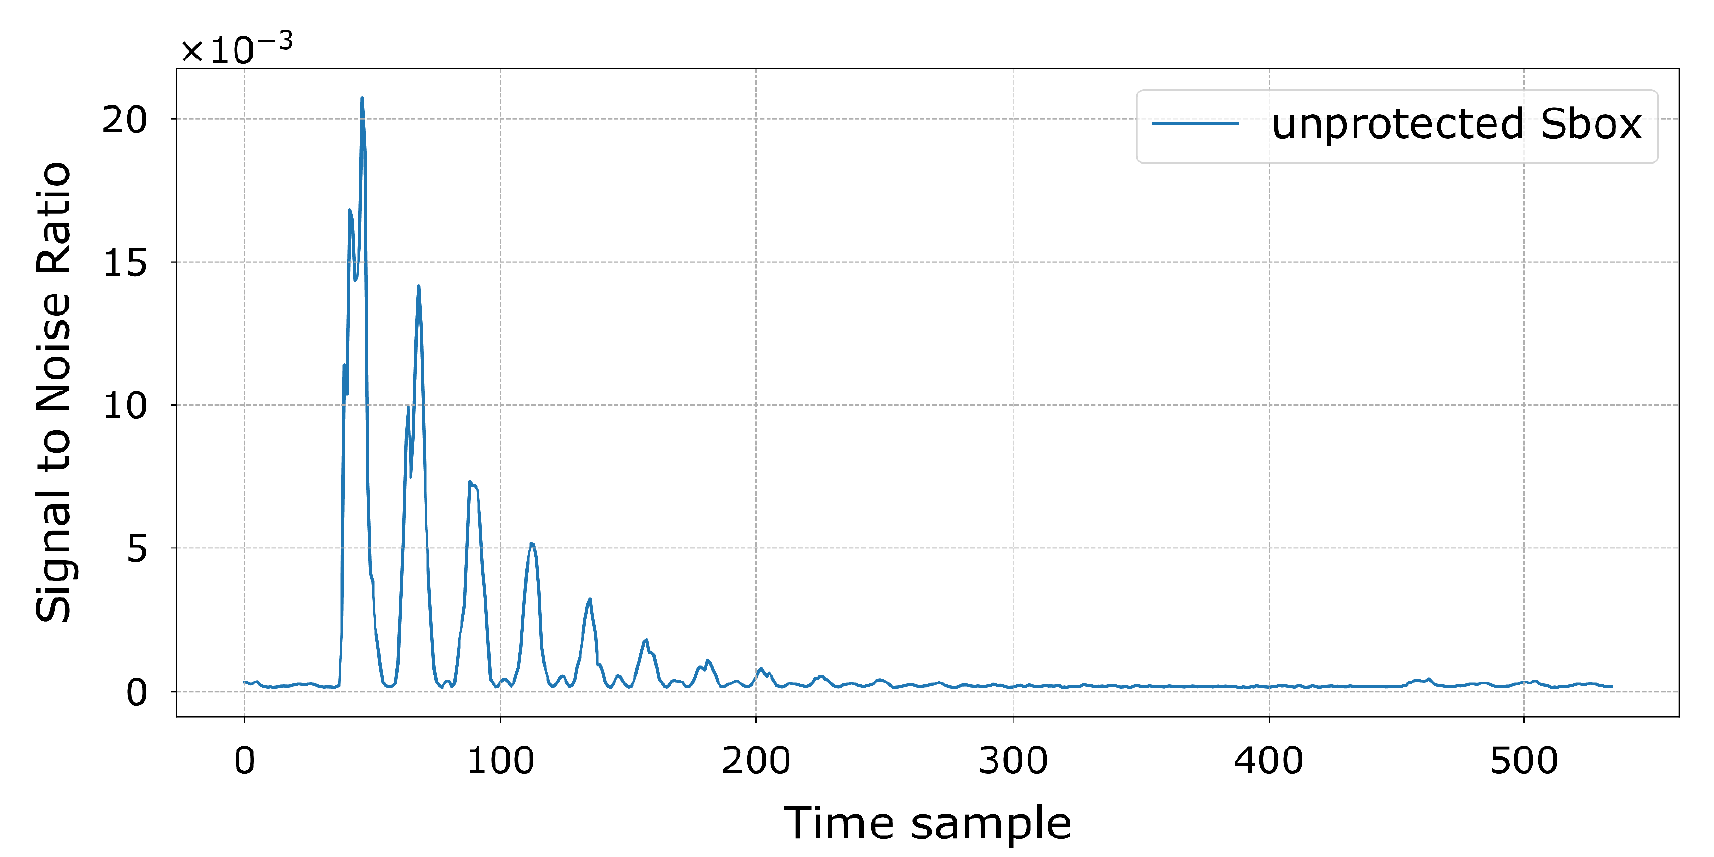
\includegraphics[width=1.0\textwidth]{metrics/Pictures/SNR_plot_unprotected_Sbox.png}
        \caption{SNR plot for an unprotected AES S-box implementation. Peaks indicate key-dependent leakage.}
    \end{figure}
\end{frame}



% Advantages and Limitations
\begin{frame}
    \frametitle{SNR: Limitations}
        \begin{itemize}
            \item \textbf{Not a direct attack feasibility metric:} It maintains a level of generality by not being tied to a specific attack method, but this also means it can't directly convey the actual security level of a device.
            \item \textbf{Simplified leakage model:} The metric implicitly relies on a simplified model of leakage (e.g., assuming a Gaussian noise distribution). In real-world scenarios, the actual leakage may diverge from these assumptions.
            \item \textbf{Parameter estimation issues:} The statistical parameters (mean and variance) must be adequately estimated from the available traces. A poor estimation due to a limited N.O.T. can lead to misleading SNR results.
            \item \textbf{Univariate nature:} The standard definition of SNR focuses on a single time sample at a time (univariate), ignoring the joint multivariate leakage that an adversary can exploit across multiple samples. 
        \end{itemize}
\end{frame}


\section{Score and Rank}

% intro
\begin{frame}
    \frametitle{Score and Rank: Why?}
    The majority of side-channel attacks employ a \textbf{divide-and-conquer} strategy. \newline
       Instead of targeting the full cipher key at once, the attack partitions it into smaller, more manageable parts. For example, a 16-byte (128-bit) AES key is typically attacked as 16 independent key bytes.
    \vspace{1cm}
    \begin{block}{The Goal}
        This approach allows the attacker to recover each small key part individually, dramatically reducing the complexity of the attack. The metrics of \textbf{score and rank} are used to evaluate the success of recovering each of these parts.
    \end{block}
\end{frame}



% Scorie and Rank Process
\begin{frame}
    \frametitle{The Scoring and Ranking Process}
    \framesubtitle{For a Single Key Part (e.g., one AES key byte)}
    For each key portion:
    \begin{enumerate}
        \item \textbf{Hypothesize:} The attacker considers all possible values for the key part. For an 8-bit key byte, this means 256 key candidates (0 to 255).
        \item \textbf{Score:} A score is computed for each key candidate. This score, generated by a distinguisher like correlation, measures how well the hypothesis for that candidate matches the observed side-channel leakage.
        \item \textbf{Guess:} The scores are sorted to produce an ordered list of guesses, from best to worst. The key candidate with the highest score becomes \texttt{guess\textsubscript{1}}, the attacker's top choice. For instance, if candidate k=42 had the best score, then \texttt{guess\textsubscript{1}} would be 42.
        \item \textbf{Rank:} A rank is assigned to each key candidate based on its position in the sorted list. The best-scoring candidate receives rank 1.
    \end{enumerate}
\end{frame}

\begin{frame}
    \frametitle{Algorithm for a Standard Attack with Score and Rank}
    
    \begin{algorithm}[H]
    \begin{algorithmic}[1] 
        \Statex \textbf{Input:} Attack score function $f(\cdot)$, Key candidates $K$
        \Statex \textbf{Data:} Simulated or real side-channel traces
        \Statex \textbf{Output:} $score_k, guess_k, rank_k$, for all $k \in K$ and all key partitions 
        %\Comment{Partition the full cipher key and attack all key parts}
        \State $partitions \gets \text{divide-and-conquer}(\text{full key})$
        \ForAll{$partition \in partitions$}
            %\Comment{Compute the attack score for every key candidate}
            \ForAll{$k \in K$}
                \State $score_k \gets f(\text{traces}, k)$
            \EndFor
            %\Comment{Sort the scores and compute the key guesses}
            \State $[score_i, score_j, \dots, score_m] \gets \text{sort}([score_0, score_1, \dots, score_{|K|-1}])$
            \State $[guess_1, \dots, guess_{|K|}] \gets [i, j, \dots, m]$
            %\Comment{Compute the rank of every key candidate using the key guesses}
            \ForAll{$guess_i$, with $i \in \{1, 2, \dots, |K|\}$}
                \State $rank_{guess_i} \gets i$
            \EndFor
        \EndFor
    \end{algorithmic}
    \end{algorithm}
\end{frame}

\begin{frame}
    \frametitle{Interpreting the Results: Convergence}
    \begin{itemize}
        \item By plotting score/rank against the number of traces, we can visualize the attack's progress.
        \item \textbf{What to look for:} A key candidate that \textbf{stands out} from the rest.
        \item A successful attack shows \textbf{convergent behavior}: one candidate consistently achieves the highest score (and thus, rank 1) as more traces are added.
        \item \textbf{Example:} Considering a CPA attack on AES-128, key candidate $K=203$ reaches rank 1 after about 15,000 traces and maintains that top position, demonstrating a successful recovery of that key byte (as shown in the following pictures). 
    \end{itemize}
\end{frame}

\begin{frame}
    \frametitle{Example: Score and Rank Plot Convergence}
    \begin{figure}
        \centering
        % Score plot
        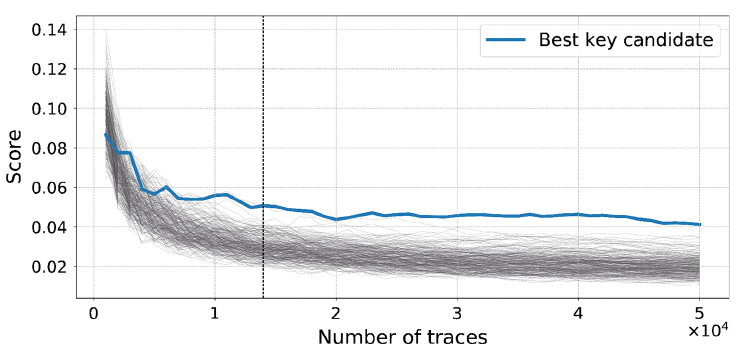
\includegraphics[width=0.55\textwidth]{metrics/Pictures/score_plot.png}
    \end{figure}
    \begin{figure}
        %\vspace{0.5cm} 
        \centering
        % Rank plot 
        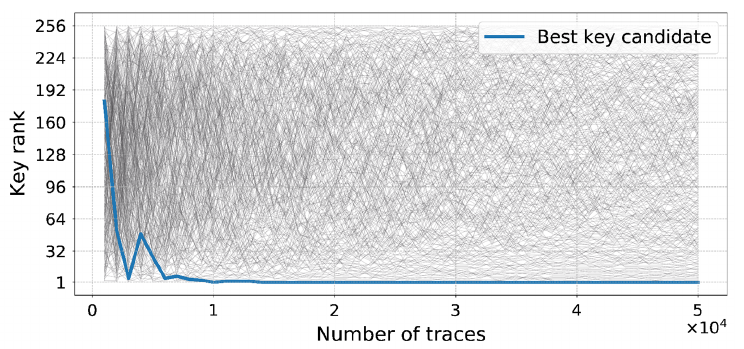
\includegraphics[width=0.55\textwidth]{metrics/Pictures/rank_plot.png}
        \caption{Top: Score plot where the correct key (K=203) is in blue\newline Bottom: Rank plot where the same key's rank converges to 1 after approx. 15,000 traces.}
    \end{figure}
\end{frame}



\begin{frame}
    \frametitle{Limitation: Statistical Stability}

    \begin{block}{The pitfall of a single experiment}
        A score/rank plot is typically generated from one traceset and one fixed key. This can be deceptive. \newline
        A single result might be an \textbf{outlier}, as some keys can be accidentally easier or harder to attack than others.
    \end{block}

        To ensure the results are meaningful, we must follow a more rigorous process:
        \begin{itemize}
            \item \textbf{Repeat} the attack multiple times.
            \item \textbf{Vary} the conditions for each run (e.g., use different keys and different sets of traces).
            \item \textbf{Aggregate} the outcomes by calculating the average score/rank and the standard deviation.
        \end{itemize}
        This gives us a \textbf{statistically stable} metric that truly reflects the device's security.
\end{frame}


\begin{frame}
    \frametitle{Limitation: The Full Key Recovery Problem}

        In a real-world attack, the key is unknown. If the attack is suboptimal or uses too few traces, the correct key parts might not achieve Rank 1. Even if the correct byte is at a low rank (like 2 or 3), the \textbf{device is still vulnerable}, but the full key remains hidden.
    
    
    \begin{block}{Key Enumeration}
        To find the full key, the attacker must perform \textbf{key enumeration}. This is a time-consuming, trial-and-error process:
        \begin{itemize}
            \item Construct full key candidates from combinations of the top-ranking key parts.
            \item Test each full key candidate (e.g., by decrypting a known ciphertext) until the correct one is found.
        \end{itemize}
        This is often a computationally expensive task.
    \end{block}
\end{frame}


\begin{frame}
    \frametitle{The Evaluator's Solution: Known-Key Analysis}

    \begin{block}{A More Efficient Approach for Evaluation}
        To assess security without the high cost of key enumeration, evaluators use a different strategy: a \textbf{known-key analysis}.
    \end{block}
    
    \begin{itemize}
        \item In this scenario, the evaluator knows the secret key from the start.
        \item This allows them to check the rank of the \textit{correct key} directly, even if the attack fails to place it at Rank 1.
        \item This answers the question "How close are we to breaking it?" and provides a more precise risk assessment than a simple pass/fail.
    \end{itemize}
    
    \begin{alertblock}{Paving the way for new metrics}
        This concept of known-key analysis is the foundation for the next metrics we will discuss: \textbf{Success Rate (SR)} and \textbf{Guessing Entropy (GE)}.
    \end{alertblock}
\end{frame}



\section{Success Rate and Guessing Entropy}


\begin{frame}
    \frametitle{Success Rate (SR) and Guessing Entropy (GE): Introduction}
    
    \begin{block}{Motivation}
        \begin{itemize}
            \item In known-key analysis, \textbf{evaluators} have access to the secret key. This allows for more precise security assessments.
            \item SR and GE metrics move beyond a simple "key recovered/not recovered" statement to quantify the attack's probabilistic progress.
        \end{itemize}
    \end{block}
    
    \begin{block}{What is Success Rate (SR)?}
        \begin{itemize}
            \item \textbf{SR} measures the probability that an attack successfully places the correct key candidate at \textbf{rank 1}.
            \item It is derived from the attack's guess vector: if the top guess (\texttt{guess\textsubscript{1}}) matches the correct key, the experiment is a success.
            \item To ensure statistical stability, SR is typically computed by averaging results over many repeated attack experiments.
        \end{itemize}
    \end{block}
\end{frame}


\begin{frame}
    \frametitle{Success Rate (SR): Definition}
    
        Recall that a standard side-channel attack produces a guess vector $[guess_1, guess_2, \dots, guess_{|K|}]$ where $guess_1$ is the best candidate. \newline
        Let $k_c$ be the correct key.    
    \begin{block}{Formal Definition}
        For a side-channel experiment $i$, the success rate $SR_i$ is 1 if the best guess equals the correct key ($guess_1 = k_c$), otherwise it's 0.
        Alternatively, using the rank of the correct key (rank $k_c$):
        $$ SR_i = \begin{cases} 1, & \text{if } rank_{k_c} = 1 \\ 0, & \text{otherwise} \end{cases} $$
        To ensure statistical stability, the final SR metric is estimated by averaging over $p$ experiments:
        $$ SR = \frac{1}{p} \sum_{i=1}^{p} SR_i $$
    \end{block}
\end{frame}


\begin{frame}
    \frametitle{Success Rate (SR): Interpretation}
    Increasing the number of attack traces typically improves the success rate gradually.
    An $SR$ value closer to 1 implies a high probability of correct key recovery. \newline % Add vertical space

    Full key recovery implies $SR=1$. However, we often want the SR metric to reflect cases where the correct key is ranked highly, yet $>$ 1. 
    \newline

    \begin{figure}[htbp]
        \centering
        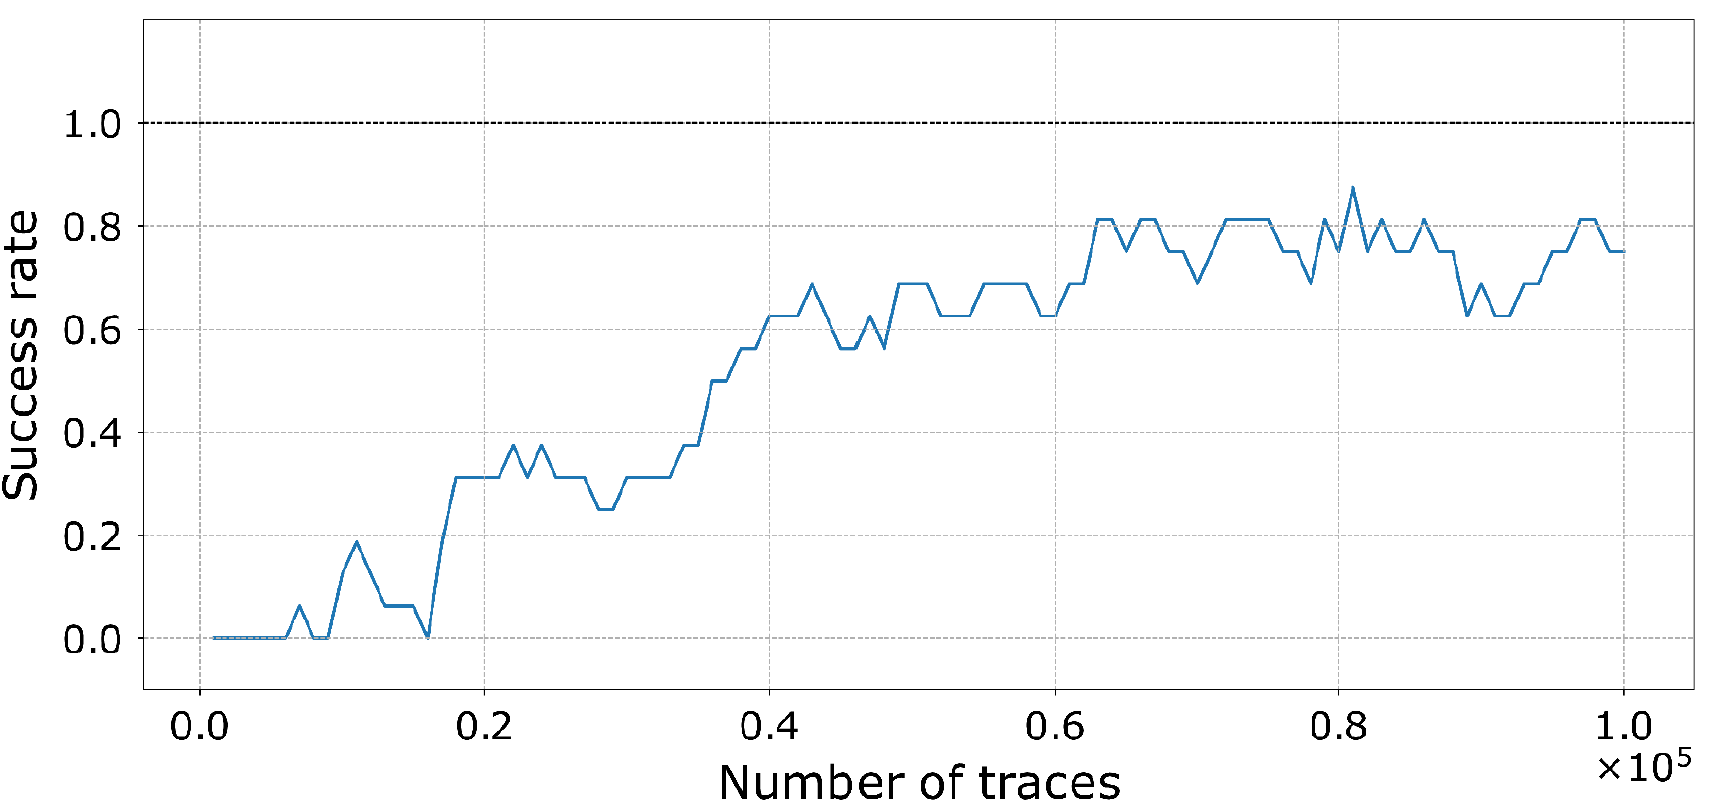
\includegraphics[width=0.8\textwidth]{metrics/Pictures/SR_plot_unprotected.png}
        \caption{for an unprotected AES using 16 parallel S-boxes, $SR$ (with 100,000 traces) is 1 only 80\% of the time}
    \end{figure}
\end{frame}
\begin{frame}
    \begin{block}{SR of Order $o$}
        The $SR$ metric can be extended to reflect cases where the correct key is ranked highly, but not necessarily 1st.
        
        $SR_i^o$ is 1 if the correct key $k_c$ is found within the top $o$ key guesses (i.e., $k_c \in [guess_1, \dots, guess_o]$ or $rank_{k_c} \le o$), otherwise 0.
        $$ SR_o^i = \begin{cases} 1, & \text{if } rank_{k_c} \le o \\ 0, & \text{otherwise} \end{cases} $$
        The overall $SR_o$ is:
        $$ SR_o = \frac{1}{p} \sum_{i=1}^{p} SR_o^i $$
        If $o=1$, this reverts to the original $SR$ definition.
    \end{block}
\end{frame}



\begin{frame}
    \frametitle{SR of Order $o$: Link to Attacker Effort}
        If an evaluator finds $SR^o=1$ for a key part, an attacker with an unknown key would need to verify at most $o$ candidates to find that key part after performing the attack.
        \newline
        \textit{Example:} If $SR^5=1$ for an AES byte, the attacker needs to check at most 5 candidates for that byte.
    
    \begin{block}{Full Key Enumeration Challenge}
        \begin{itemize}
            \item This key enumeration process must be repeated for all divide-and-conquer partitions of the full key.
            \item For example, if $SR^5=1$ for all 16 AES-128 key bytes, an attacker might need to verify up to $5^{16}$ full keys.
            \item This is a computationally challenging, heuristic task, and determining the appropriate value for $o$ is critical for assessing attacker capability.
        \end{itemize}
    \end{block}
\end{frame}


\begin{frame}
   
    \frametitle{Guessing Entropy (GE): Definition}
    
        To avoid the heuristic and potentially complex process of $SR$ of order $o$ for full key enumeration, Guessing Entropy (GE) offers a more flexible metric.
   
    
    \begin{block}{GE Formal Definition}
        Given a rank vector $[rank_0, rank_1, \dots, rank_{|K|-1}]$ and the correct key $k_c$, the rank of $k_c$ ($rank_{k_c}$) can be found and plotted against the number of traces.
        
        For a given experiment $i$, $GE_i$ is defined as:
        $$ GE_i = \log_2(rank_{k_c}) $$
        It is typically expressed in bits.
        
        The overall GE, averaged over $p$ experiments (where $k_c$ is ideally changed between experiments to ensure statistical stability), is:
        $$ GE = \frac{1}{p} \sum_{i=1}^{p} GE_i $$
    \end{block}
\end{frame}



\begin{frame}
    \frametitle{Guessing Entropy (GE): Interpretation and Example}

        The $rank_{k_c}$ and GE metrics represent the average remaining workload for an attacker after a side-channel attack.
        GE = 0 means the side-channel attack has eliminated all uncertainty about the secret key
            %\item For masked S-box implementations, GE stays substantially above 0 (about 8 bits even with 50,000 traces), showing that the attack leaves significant uncertainty and the device remains resistant.

    \begin{figure}
        \centering
        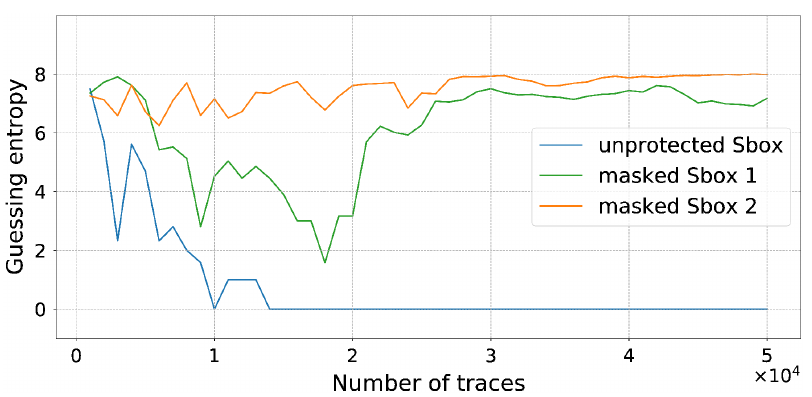
\includegraphics[width=0.75\textwidth]{metrics/Pictures/GE_plot.png}
        \caption{Guessing Entropy plot for three AES S-box implementations. GE drops to 0 for the unprotected S-box after roughly 15,000 traces; for masked S-boxes, GE remains high even with 50,000 traces.}
    \end{figure}
\end{frame}

%%%%REVIEW
\begin{frame}
    \frametitle{Limitations of SR and GE: Full Key Security}

    \begin{block}{Byte-wise Metrics Do Not Translate Directly}
        Both Success Rate (SR) and Guessing Entropy (GE) quantify attack effectiveness for individual key bytes (e.g., in AES). However, knowing the GE or SR for all bytes does \textbf{not} allow direct inference of the GE or SR for the full key.
    \end{block}

    \begin{itemize}
        \item The process of full key recovery requires \textbf{key rank estimation}, which is the known-key analog of key enumeration.
        \item Full key security assessment is more complex than simply combining values for each byte; detailed estimation methods are required.
    \end{itemize}
\end{frame}

\begin{frame}
    \frametitle{Limitations of SR and GE: No Projection of Effort}

    \begin{block}{Trace-Dependency Limits Security Forecast}
        SR and GE provide attack progress for a specific number of measured traces, but do not project future effort required for successful key recovery.
    \end{block}

    \begin{itemize}
        \item If SR or GE is close to random guessing (e.g., 1/256 for AES byte), one can only conclude the attack currently fails.
        \item The metrics do \textbf{not} indicate how many more traces would be needed to break the cipher, nor are they designed to forecast eventual success.
        \item GE is an expression of the remaining effort, but it is always derived from a specific number of measured traces.
    \end{itemize}

    \begin{block}{Towards Better Projections}
        This limitation led to the development of new metrics, which tie attack scores and success probabilities more rigorously to the number of traces.
    \end{block}
\end{frame}






\end{document}